%sekcja wyboru czujnika piezo
\section{Selekcja czujnika}
\label{sec:sensor_selection}
Równolegle z pracami nad stanowiskiem badawczym przeprowadzono przegląd dostępnych na rynku przetworników piezoelektrycznych. Uwagę skoncentrowano przede wszystkim na przetwornikach PVDF\cite{PVDF:15}\footnote{Polifluorek winylidenu - materiał piezoelektryczny charakteryzujący się elastycznością.} Do badań wybrano 6 konkretnych produktów (patrz: Rys.\ref{fig:sensors}.):

\begin{enumerate}
\item Czujnik TODO
\item Czujnik TODO
\item Czujnik TODO
\item Czujnik TODO
\item Czujnik TODO
\item Czujnik TODO
\end{enumerate}


\begin{figure}[htbp]
\centering
\fbox{TUTAJ ZDJĘCIE CZUJNIKÓW}%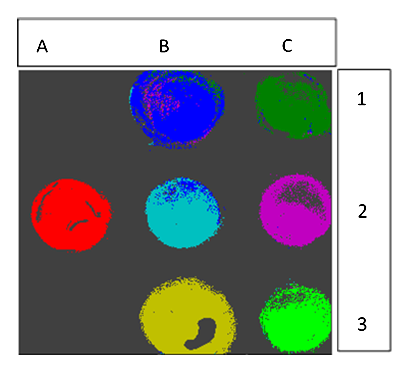
\includegraphics[width=\linewidth]{sample}}
\caption{Badane przetworniki piezoelektryczne.}
\label{fig:sensors}
\end{figure}

Aby dokonać selekcji przetwornika wybrano najprostszy układ geometryczny (patrz: Rys. \ref{fig:sensor_sel_geometry}). Został on wykonany z fragmentu tworzywa sztucznego. Układ oznaczono tak, aby można było ustawić go ponownie w tej samej pozycji po wymianie sensora. Sensor przyklejano na taśmę dwustronną o grubości ok w ustalonym uprzednio miejscu. $1.5mm$. 

\begin{figure}[htbp]
\centering
\fbox{TUTAJ RYSUNEK GEOMETRII CZUJNIKA }%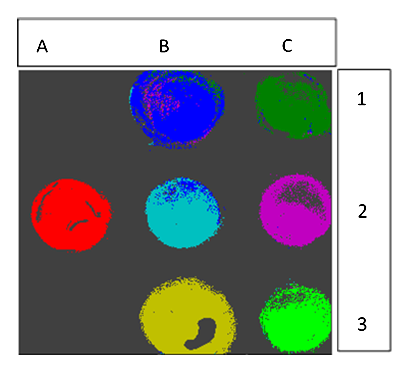
\includegraphics[width=\linewidth]{sample}}
\caption{Konstrukcja pozwalająca na selekcję przetwornika piezoelektrycznego.}
\label{fig:sensor_sel_geometry}
\end{figure}

Dla uzyskania szerszego spektrum danych dla każdego czujniaka powtarzano poamiary w dwóch wariantach: 
\begin{enumerate}
\item stała podpora na jednym z końców układu przetwornika, drugi koniec swobodny,
\item stała podpora na jednym z końców układu przetwornika, drugi koniec z amortyzatorem z gąbki.
\end{enumerate}
Dla każdego pomiaru przeprowadzono po 10 prób, i pozwoliło to zebrać poniższe wyniki. Parametry, jakie wzięto pod uwagę przy ocenie jakości sygnału, to czas trwania ( od inicjalizacji do wygaszenia ) oraz wartość napięcia międzyszczytowego oznaczanych dalej odpowiednio $t_d$ i $V_{pp}$. Ich porównanie po statystycznej analizie przedstawiono na Rys.\ref{fig:sensor_sel_geometry}. Trzeci niebieski słupek w skali od $0\div5$ oznacza subiektywną ocenę poziomu zniekształcenia otrzymanego sygnału. Podczas badań zwracano również uwagę na sposób przyklejenia przetwornika do plastikowego płaskownika tak, aby nie fałszowało to przeprowadzanych pomiarów. 
%TODO Tu przydałby się rozkład widmowy sygnału

\begin{figure}[htbp]
\centering
\fbox{TUTAJ WYKRES PORÓWNAWCZY SYGNAŁÓW }%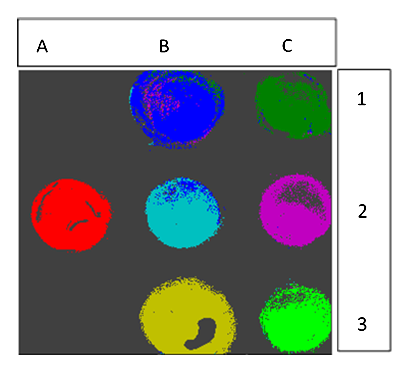
\includegraphics[width=\linewidth]{sample}}
\caption{Zestawienie parametrów sygnałów dla poszczególnych czujników.}
\label{fig:sensor_sel_geometry}
\end{figure}

Na podstawie Rys.\ref{fig:sensor_sel_geometry} możemy stwierdzić, że najwyższą wartość uzyskanego napięcia $V_{pp}$ otrzymaliśmy dla czujnika oznaczonego numerem 1.2. Szacuje się, że wyższa wartość $V_{pp}$ będzie bradziej odporna na szumy pochodzące z maszyny, na której sensor byłby umieszczony. Zgodnie z założeniami przeznaczeniem sensora jest przecież licznik impulsów mechanicznych. Z dużym prawdopodobieństwem można uznać, że wyzwalanie licznika następować będzie na jednym ze zboczy pierwszej półfali lub np. wyprostowanej całej fali sygnału. 
\ident Odnośnie czasu trwania sygnału jednoznacznie można stwierdzić, że im krótszy tym lepszy. Pozwala to na zwiększenie częstotliwości występowania wymuszeń mechanicznych bez wystąpienia zjawiska aliasingu.


